\SECTION{دنباله و اعداد فیبوناچی}
\begin{EXTRA}{ فیبوناچی }
\p
\centerimage{0.2}{./Leonardo.jpeg}
Pisa
of 
Leonardo
معروف به
فیبوناچی، ریاضیدان ایتالیایی قرن 
۱۳
است.
پدر او تاجر بوده و به همراه پسرش سفرهای زیادی به خاورمیانه داشته است.
فیبوناچی ریاضیات را از عرب‌ها آموخت.
در آن زمان غربی‌ها از سیستم اعداد رومی استفاده می‌کردند اما اعراب سیستمی نزدیک به امروز داشتند.
استفاده کردن از اعداد رومی بسیار پیچیده‌ و فاقد صفر بودند، به این ترتیب پیشرفت علم ریاضی را با مشکل مواجه کرده بود.
فیبوناچی در سال ۱۲۰۲ با انتشار کتاب
Abaci
Liber
آغاز به
گسترش استفاده از سیستم اعداد جدید کرد.
در این کتاب فیبوناچی مسئله زاد و ولد خرگوش‌ها را مطرح کرد. (در مثال زیر آن را بررسی می‌کنیم.)
بعدها این مسئله موجب به وجود آمدن دنباله پرکاربرد فیبوناچی شد.
هر چند مسئله خرگوش‌ها ساختگی بود اما در طبیعت، بسیاری از جانوران مانند زنبورها و گیاهان از این الگوی رشد جمعیت تبعیت می‌کنند.
در بیشتر بدانید بعدی در مورد کاربرد دنباله فیبوناچی در طبیعت صحبت می‌کنیم.
\end{EXTRA}

\subfile{./rabbitsProblem.tex}

\NOTE{توجه کنید به تعداد جملاتی که در رابطه بازگشتی به عقب برمی‌گردیم به جملات پایه نیاز داریم.
در تعریف دنباله‌ فیبوناچی چون
$f_{n-1}$
    و
    $f_{n-2}$ 
    داريم دو جمله پایه
    $f_{1} = 1$
    و
    $f_{2} = 1$
    را تعریف کردیم.  }
    
\begin{DEFINITION}
    به اعدادی که در رابطه بازگشتی
  \[\begin{cases}
      f_{n}=f_{n-1} + f_{n-2} & n\geq 2 \\
      
      f_0=1 ,
      f_1 = 1
  \end{cases}
  \]
  صدق می کنند,
  \FOCUSEDON{  دنباله‌ فیبوناچی}
    می‌گوییم.
    به عبارتی دنباله فیبوناچی
    دنباله‌ای از اعداد است که در آن به جز دو جمله اول، هر جمله از مجموع دو جمله‌ی قبلی به دست می‌آید.
    \p
  $$1, 1, 2, 3, 5, 8, 13, 21, 34, 55, 89, ...$$
\end{DEFINITION}


\subfile{./example1.tex}

\begin{THEOREM}
    \p
    \FOCUSEDON{تابع مولد دنباله فیبوناچی}
    برابر است با:
    $$F(x) = \frac{1}{1 - x - x^2}$$
    \FOCUSEDON{فرمول صریح فیبوناچی}
    برابر است با:
    $$f_n = \frac{1}{\sqrt{5}}((\frac{-1 + \sqrt{5}}{2})^{n} - (\frac{1 - \sqrt{5}}{2})^{n})$$
\end{THEOREM}

\subfile{./example2.tex}

\begin{EXTRA}{ فیبوناچی در طبیعت}
  \p
دنباله فیبوناچی خواص شگفت‌انگیزی دارد که باعث می شود در آثار برجسته هنر و معماری، دانه‌های گل آفتاب گردان، صدف‌ها و تولید مثل خرگوش‌ها و زنبورها، آثار آن دیده شود.
فیبوناچی در کتاب خود 
Abaci
Liber
 اثر آن در تولید مثل خرگوش‌ها را بیان کرده است و در مثال‌های بالا این مسئله را بررسی کردیم. حال به بررسی چند مسئله واقعی دیگر که فیبوناچی تاثیرگذار بوده است می‌پردازیم.
\p
مارپیچ فیبوناچی:
با قرار دادن مربع‌هایی به ضلع اعداد فیبوناچی در کنار هم و اتصال رئوس این مربع‌ها به کمک کمان، مارپیچ فیبوناچی تشکیل می‌شود.
\p
\centerimage{0.4}{./Fibonacci.jpeg}
\p
اعداد فیبوناچی در هستی کشف شده‌اند.
لاک حلزون
 دریایی دقیقا با الگوی مارپیچ فیبوناچی به وجود آمده است. موقعیت اهرام مصر نسبت به هم، حرکت گردباد روی زمین، نحوه رشد گلبرگ ها و دانه‌های آفتابگردان و کهکشان‌ها منطبق بر مارپیچ فیبوناچی هست.
 درختان با پیروی از این نوع الگوی رشد، قادرند درصد بیشتری از نور خورشید را جذب کنند.

 \p
 در شکل زیر اگر گیاه از هر گره ۲ ماه زمان لازم داشته باشد تا دوشاخه شود می‌بینیم در پایان هر ماه تعداد ساقه‌ها اعداد فیبوناچی هستند.
 \centerimage{0.4}{./sneezewort.jpeg}

\p
در اکثر گل‌ها تعداد گلبرگ‌ها ۳ ، ۵ ، ۸ ، ۱۳ و .. است.
% \begin{figure}
%   \centering
%   \subfloat[]{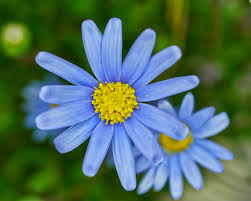
\includegraphics[width=0.24\textwidth]{flower1.jpeg}} 
%   \subfloat[]{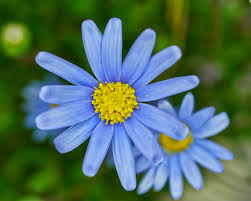
\includegraphics[width=0.24\textwidth]{flower1.jpeg}} 
%   \subfloat[]{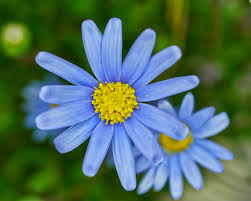
\includegraphics[width=0.24\textwidth]{flower1.jpeg}}
%   \subfloat[]{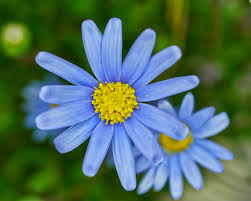
\includegraphics[width=0.24\textwidth]{flower1.jpeg}}
%   \caption{(a) blah (b) blah (c) blah (d) blah}
%   \label{fig:foobar}
% \end{figure}

\centerimage{0.4}{./flower1.jpeg}
\centerimage{0.4}{./flower2.jpeg}
\centerimage{0.4}{./flower3.jpg}
\p
حتما با عدد طلایی آشنا هستید. نسبت طلایی به روش‌های متفاوتی به دست می‌آید. جالب است بدانید نسبت هر دو جمله متوالی از دنباله فیبوناچی به عدد طلایی میل می‌کند.
اگر نسبت عدد چهلم این رشته را به عدد قبلی حساب کنیم به عدد $ 1.618033988749895$ می‌رسیم که با تقریب ۱۴ رقم اعشار نسبت طلایی را نشان می‌دهد.
\p
نسبت طلایی ($1.618$) در آناتومی بدن انسان نیز بکار رفته است. اگر قد خود را بر فاصله عمودی ناف تا نوک انگشتان خود تقسیم کنید، تقریبا عدد $1.618$ را بدست می‌آورید. با تقسیم طول بازوی خود از نوک انگشت بزرگ تا بالای شانه، بر فاصله نوک انگشت بزرگ تا آرنج خود نیز به این نسبت می‌رسید .
\p
علاوه بر طبیعت، از زمان باستان بسیاری از هنرمندان و معماران نیز از رابطه‌های ریاضی و هندسی در آثار خود استفاده می‌کردند. برای مثال می‌توان به آثار تاریخی باقی مانده از دوران مصر باستان، یونان و رم اشاره کرد. مثلا معبد معروف پارتنون بهترین مثال از کاربرد نسبت طلایی ($1.618$) است. نسبت عرض به طول پنجره‌های مستطیل شکل معبد همگی برابر نسبت طلایی است. در اهرام مصر نیز این نسبت به خوبی رعایت شده است. طول هر ضلع قاعده هرکدام از اهرام به ارتفاع آن، معادل نسبت طلایی می‌باشد.

\end{EXTRA}